% Diagram: Transformer Parallel Processing
\begin{figure}[htbp]
\centering
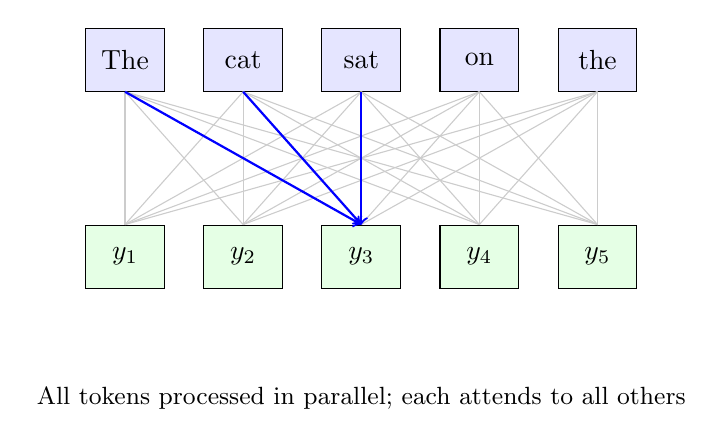
\begin{tikzpicture}[
    node distance=1.5cm,
    token/.style={rectangle, draw, minimum width=1cm, minimum height=0.8cm, fill=blue!10},
    output/.style={rectangle, draw, minimum width=1cm, minimum height=0.8cm, fill=green!10},
    arrow/.style={->, thick}
]
% Input tokens
\node[token] (t1) {The};
\node[token, right of=t1] (t2) {cat};
\node[token, right of=t2] (t3) {sat};
\node[token, right of=t3] (t4) {on};
\node[token, right of=t4] (t5) {the};

% Output representations
\node[output, below of=t1, yshift=-1cm] (o1) {$y_1$};
\node[output, below of=t2, yshift=-1cm] (o2) {$y_2$};
\node[output, below of=t3, yshift=-1cm] (o3) {$y_3$};
\node[output, below of=t4, yshift=-1cm] (o4) {$y_4$};
\node[output, below of=t5, yshift=-1cm] (o5) {$y_5$};

% Attention connections (showing each output attends to all inputs)
\foreach \i in {1,2,3,4,5} {
    \foreach \j in {1,2,3,4,5} {
        \draw[gray!40, thin] (t\j.south) -- (o\i.north);
    }
}

% Highlight one token's attention pattern
\draw[blue, thick, ->] (t1.south) -- (o3.north);
\draw[blue, thick, ->] (t2.south) -- (o3.north);
\draw[blue, thick, ->] (t3.south) -- (o3.north);

% Labels
\node[below of=o3, yshift=-0.3cm] {\small All tokens processed in parallel; each attends to all others};
\end{tikzpicture}
\caption{Transformer processing: all tokens processed simultaneously with direct attention connections.}
\label{fig:transformer-parallel}
\end{figure}
